% !TEX root=./whitepaper.tex
\section{System Design}

\project employs layered design targetting to support different types of decentralized applications. Figure~\ref{fig:stack} shows the overview of the full stack layers of \project system. 

\begin{figure}[H]	
	%\vspace{-6mm}
	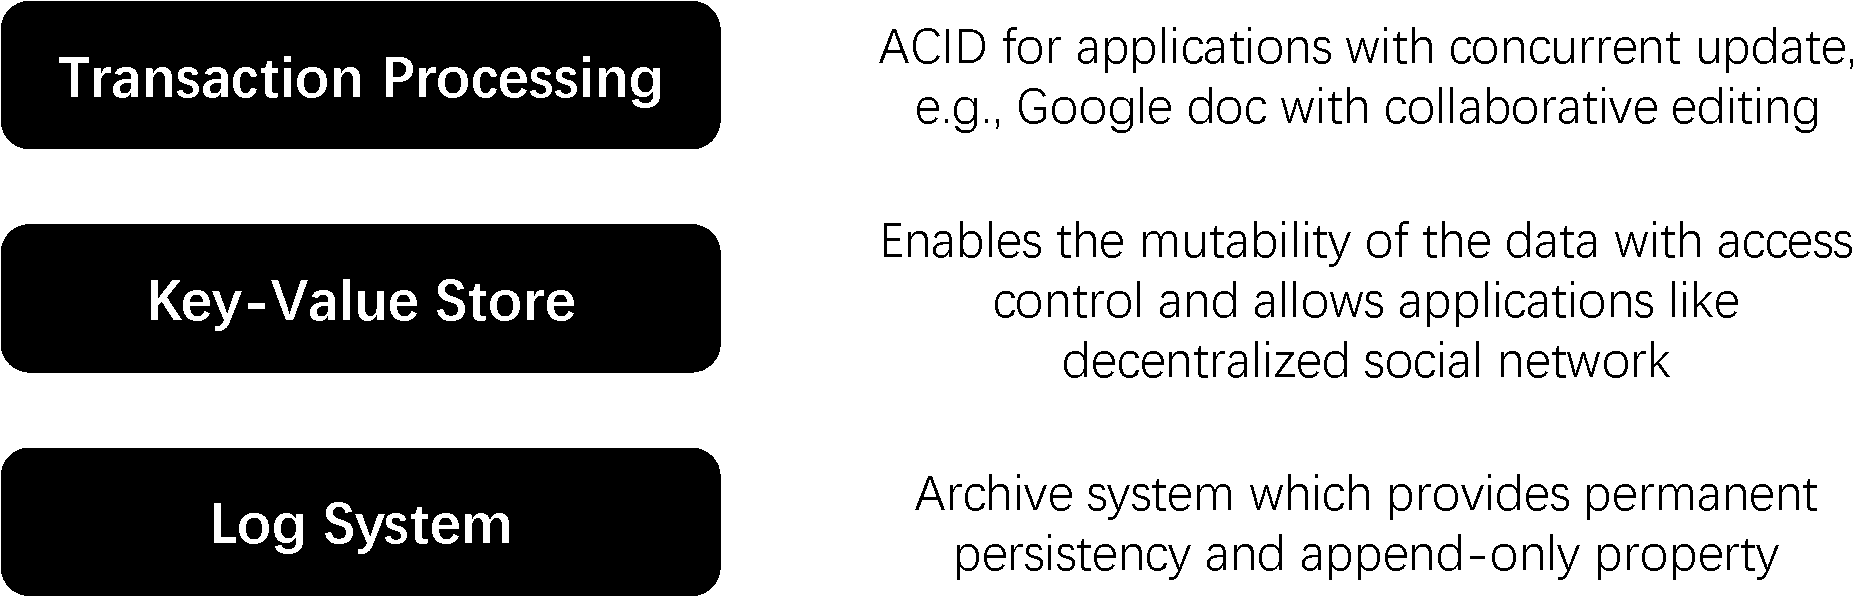
\includegraphics[width=\textwidth]{figure/stack-crop.pdf}
	\caption{Full Stack Solution of Ionian}
	\label{fig:stack}
	%\vspace{-10mm}
\end{figure}

The lowest is a log layer that is a decentralized system. It consists of multiple storage nodes to form a storage network. The network has built-in incentive mechanism to reward the data storage. The ordering of the uploaded data is guaranteed by a sequencing mechanism to provide a log-based semantics and abstraction. This layer is used to store unstructured raw data for permanent persistency.

On top of the log layer, \project provides a Key-Value store runtime to manage structured data with mutability. Multiple key-value store nodes share the underlying log system. They put the structured key-value data structure into the log entry and append to the log system. They play the log entries in the shared log to construct the consistent state snapshot of the key-value store. The throughput and latency of the key-value store are bounded by the log system, so that the efficiency of the log layer is critical to the performance of the entire system. The key-value store can associate access control information with the keys to manage the update permission for the data. This enables the applications like social network, e.g., decentralized Twitter, which requires the maintenance for the ownership of the messages created by the users. 

\project further provides transactional semantics on the key-value store runtime to enable concurrent updates for the keys from multiple users who have the write access permission. The total order of the log entries guaranteed by the underlying log system provides the foundation for the concurrency control of the transactional executions on top of the key-value store. With this capability, \project can support decentralized applications like collaborative editing and even database workloads.    
